\subsection{Relational databases}
The group last year chose to implement the \texttt{WordCount} and \texttt{Fuseki} databases using PostgreSQL.
PostgreSQL is a relational database system \cite{knox2020}.


A relational database consists of several layers.
The lowest level is the physical layer which describes how the data is stored physically.
The purpose of the relational model is to abstract over the physical layer of the database.
This abstraction is known as the logical layer and allows database administrators to manage the physical storage without directly manipulating the physical data representation.
The logical layer describes what data is stored and the relationships between the data.
The highest of abstraction is the view layer which describes only part of the database. It exists to simplify the interaction with the system. Many views may exist for the same database.
\cite[Chapter 1.3]{DBSBook}

Compared to storing data on a regular file system, a database system provides many advantages including atomicity of operations, concurrent access to data, and lowered inconsistency and redundancy of data \cite[Chapter 1.2]{DBSBook}.
These advantages can be directly seen in the ACID properties that databases adhere to when performing a transaction \cite[Chapter~17]{DBSBook}.
\begin{itemize} \label{ACID}
    \item Atomicity: A transaction must either be fully completed or partial side-effects of a failed transaction must be undone.
    \item Consistency: A transaction in isolation must ensure values remain consistent after a transaction has been completed or terminated.
    \item Isolation: Transactions are unaware of other transactions being executed concurrently to avoid confusion.
    \item Durability: Changes caused by a committed transaction persist even in the event of system failures.
\end{itemize}

In the coming sections, we will describe how one can model and describe a relational database design, both mathematically and with a more graphic design.
After doing this, we will examine how operations on these models can be described using SQL and relational algebra.

\subsubsection*{Relational model}
Relational database systems can be mathematically described using relations and sets, mapping a unique key to a tuple of information \cite[Chapter~2.3]{DBSBook}.
The values of the tuples contained within the relation can be described by the attributes of the relation and their corresponding domains \cite{KatjaFirstPP}. 
The relations are often described using a \textit{relational schema}, denoting the name and domains of the attributes.


Equation \ref{eq:relational_schema} shows an example of a relation describing books as tuples of three text fields (author\_name, title, and ISBN) and a positive integer (number\_of\_pages).
The relation also denotes a super key for the relation. A super key is one or more attributes that can uniquely identify a tuple in a given relation.
Any super key, where if just one attribute is removed it does no longer uniquely identify tuples, is called a \textit{candidate key}.
Attributes describing the super key are underlined.

\begin{equation} \label{eq:relational_schema}
    book(author\_name:text, title: text, number\_of\_pages:\mathbb{Z}^+, \underline{ISBN: text})
\end{equation}
Super keys can be defined as $t_1 \in r,\neq t_2 \in r \implies t_1.K \neq t_2.K$. 

That is, no two tuples $t_1, t_2$ from relation $r$ have same values for all super key attributes $K$. 
If the super key does not contain extraneous attributes, it is said to be \textit{minimal}. \cite[Chapter 2.3]{DBSBook}
We will use the term \textit{primary key} to denote a chosen super key of a relation. 
When describing a database, it is often necessary to specify how various data are connected. 
To do this, one can use \textit{foreign keys} to denote that tuples in $r_1$ are related to the tuples in $r_2$.


One could model the relationship between a book owner and a book using the relational schemas seen in equation \ref{eq:bookOwnerExample} and \ref{eq:relational_schema}.
There, primary keys from other relations are used to reference unique tuples. The $owns$ relation describes how relations $book$ and $book\_owner$ are connected. 
\begin{equation}\label{eq:bookOwnerExample}
    \begin{split}
        owns(\underline{owner\_id \rightarrow book\_owner}, \underline{ISBN \rightarrow book}), \\
        book\_owner(name:text,\underline{owner\_id:\mathbb{Z}^+})
    \end{split}
\end{equation}

Instead of describing the data structures of the database in these relations, one can use a different model that represents the logic of the relational schemas.

\subsubsection{Entity relationship model}\label{sec:EntityRelationModel}
The entity relationship model is a graphical representation of how database relations are structured.
This is done in a \textit{E-R diagram}, and is commonly used facilitate database design from specifications of enterprise schemas \cite*[Chapter 6.2]{DBSBook}.
However, in the E-R model we differentiate between \textit{entity sets} representing domain elements and \textit{relationships sets} representing the connections between the domain elements. 
The entity sets are represented graphically with a rectangle and relationship sets connecting the entity sets with a diamond \cite[Chapter 6.2]{DBSBook}.
The attributes associated with the entity- and relationship sets can be modelled using ovals \cite{KatjaFirstPP}, however other alternatives exists.\footnote{Our style of choice is presented in Chapter 6.10 of \citetitle{DBSBook} \textit{\citefield[]{DBSBook}[]{edition}}}
Similar to the relational model, the entities (tuples) must be uniquely identified by one or more attributes. This is denoted by underlining the attributes. 

The E-R model have notations that denotes the participations each entity have in a connecting relationship \cite[Chapter 6.4]{DBSBook}.
In this project, we will use \text{min-max} notation; this notation denotes the minimum and maximum amount of entities participating in a relationship. 

\begin{figure}[htp]
    \centering
    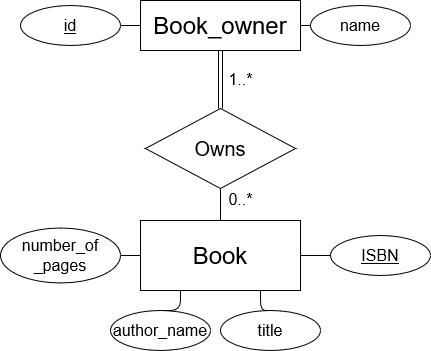
\includegraphics[scale=0.5]{Images/book_example_w_cardinality.png}
    \caption{E-R diagram of the book and book owner example.}
    \label{fig:ER_Book_Example}
\end{figure}

Figure \ref{fig:ER_Book_Example} shows an E-R diagram equivalent to the $book$, $owns$, and $book_owner$ relations from equation \ref{eq:bookOwnerExample} and \ref{eq:relational_schema}.
In figure \ref{fig:ER_Book_Example} we also see the  the participation cardinalities of the two entity sets. 
The relationship from $book\_owner$ to $owns$ is one of total participation. That is, each book owner entity must own at least one book.
\begin{figure}[h]
    \centering
    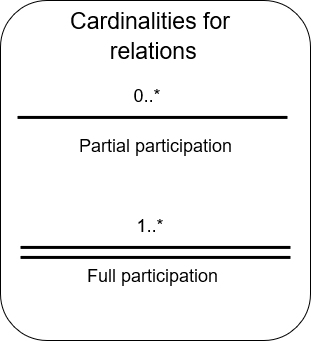
\includegraphics[scale=0.5]{Images/cardinalities.png}
    \caption{Participation ratios for ER relationships}
    \label{fig:ERDiagram_Cardinality}
\end{figure}
The participation from $book$ to $owns$ is partial. Thus the model represents that books can be in the database, even if no one owns it, that a book can be owned by multiple book owners.
Participation connections can be seen on figure \ref{fig:ERDiagram_Cardinality}.


Other forms of entity sets exits. For instance, a weak entity set, denoted by a an oval with doubled edges, is an entity sets whose existence is based on another entity set. Relationship sets connecting a weak entity set to its' identifying entity set will not have any attributes.
A weak entity set is identified by its \textit{identifying entity set}'s primary key along with extra attributes. 
The relationship between weak entity sets and its identifying set is always many-to-one with total  participation of the weak entity set.

Since the relational model is described using relations, we can also describe operations that can be performed on the relations.
Therefore, it is useful to be able to convert an E-R model into an equivalent relational model, where domains of attributes can be well defined and operations on the entity sets described mathematically.

\subsubsection*{Converting E-R models to relations}
\textbf{Strong entity sets}\\
Strong entity sets are converted by taking each attribute of the entity set, and a relation with corresponding attributes. 
The primary key of the entity set is chosen as primary key for the relation \cite[Chapter 6.7.1]{DBSBook}.\\
\textbf{Many-to-many relationships}
When converting many-to-many relationships to a relation, one create a single relation with primary key attributes from the participating entity sets \cite[Chapter 6.7.1]{DBSBook}. These keys are used as foreign key to reference the converted entities participating in the relationship. 
The remaining attributes of the entity set is similarly mapped to the relation.\\
\textbf{Many-to-one relationships}
If we have a many-to-one relationship between two sets we can combine the relationship set and the relation created from the entity set on the 'many' side into a single relation. This relation will use the primary key of the entity set as its primary key, and have a foreign referencing the relation created from the 'one' side of the relationship.\\
\textbf{One-to-one relationships}
When converting one-to-one relationships with total participation, we simply create a union of the attributes of the participating entity sets and the relationship set \cite[Chapter 6.7.6]{DBSBook}. If there is not total participation, two relations are created from the entity set, and a foreign key is placed on one of the sets.\\
\textbf{Weak entity sets}
When representing weak entity sets, one creates a relation containing the attributes of the weak entity set as well as the attributes of the identifying set's primary key.
The primary key of the identifying relation will also serve as a foreign key to the identifying relation. \cite[Chapter 6.7.1]{DBSBook}.
The relationship set is simply ignored, as the relationship set will not have any attributes \cite[Chapter 6.7.5]{DBSBook}. 


\subsubsection{Relational algebra}\label{sec:relationalAlgebra}
Relational algebra describes a set of unary and binary operations on relations that produce new relations.
The operations are used to define new relations, often the tuples within the set will satisfy defined predicates.
The relational operators form the foundations of data manipulation languages (see Section \ref{sec:SQL}) which can be used to define database operations \cite[Chapter 6.2]{DBSBook}.


\begin{table}[h]
    \centering
    \begin{tabular}{|lll|}
    \hline 
    \multicolumn{1}{|l|}{\textbf{Operator}}          & \multicolumn{1}{l|}{\textbf{Example}}   & \multicolumn{1}{l|}{\textbf{Is unary}}      \\ \hline
    \multicolumn{1}{|l|}{Select}                     & \multicolumn{1}{l|}{$\sigma_{predicate}(R)$}             & \multicolumn{1}{l|}{$\checkmark$}           \\ \hline
    \multicolumn{1}{|l|}{Projection}                 & \multicolumn{1}{l|}{$\pi_{A_1, A2,...,A_n}(R)$}             & \multicolumn{1}{l|}{$\checkmark$}           \\ \hline
    \multicolumn{1}{|l|}{Join}                 & \multicolumn{1}{l|}{$r_1 \Join_\Theta r_2$}             & \multicolumn{1}{l|}{$\times$}           \\ \hline
    \multicolumn{1}{|l|}{Cartesian product}          & \multicolumn{1}{l|}{$r_1\times r_2$}              & \multicolumn{1}{l|}{$\times$}            \\ \hline
    \end{tabular}
    \caption{Table of operators}
    \label{Relational algebra operators}
\end{table}

We will describe some of the operators of relational algebra, and use them to describe implemented queries later.
Some of the common operators of in relational algebra can be seen on table \ref{Relational algebra operators}.\\
\textbf{Select}\\
The select operator defines a set, $R_{result}\subseteq R$ where all tuples $t \in R_{result}$ satisfies a given predicate \cite[Chapter 2.6.1]{DBSBook}.\\
That is, $\forall t \in R_{result} \vDash predicate$.\\
\textbf{Projection}\\
The projection operator specifies a relation containing only a subset of the attributes of the operand relation \cite[Chapter 2.6.2]{DBSBook}.
That is, attributes $A_1, ..., A_n$ of relation $R_{result}$ will be a subset or equal to the attributes of the operand.\\
\textbf{Cartesian product}\\
The cartesian product of two relations $R_1$ and $R_2$ produces a set containing concatenated tuples of the two operands.
That is, taking the attributes of the two sets, $A_1,...,A_n \in R_1$ and $A_{n+1},...,A_k \in R_2$ produces a set with attributes $A_1,...,A_k$.
If the attributes of the operands have the same names we distinguish between them  by denoting their original relation: $R_1.AttributeName$, $R_2.AttributeName$. \cite[Chapter 2.6.4]{DBSBook}\\   
\textbf{Join}\\
The join operator defines a relation consisting of tuples from the cartesian product of the operand, containing only tuples satisfying the given predicate.
Thus it is defined as $\sigma_{\Theta} (R_1 \times R_2)$ \cite[Chapter 2.6.5]{DBSBook}.

As we have now established both how to model database relations as well fundamental operations used to extract data (tuples) from these relations, we can now look at how to implement the relations in a database.

\subsubsection{SQL}\label{sec:SQL}
SQL is one of the most commonly used data definition language (DDL) and data manipulation languages (DML) \cite[Chapter 3.1]{DBSBook}.
SQL is a declarative query language, where one executes a query to instruct the database system to perform a set of operations to compute a desired result. 
Collectively, the resulting set of operations is known as a transaction.
In PostgreSQL, all queries, both to define and to manipulate data, are executed as transactions \cite{postgres_transactions}.
As a DDL, SQL provides queries to define and modify relation schemas, as well as provide constraints for the attributes of the schema, such that data in the relation satisfies the constraint.  

\begin{lstlisting}[
    label=lst:CreatingTablesInSQL,
    language=SQL,
    caption=Implementing the relations from in equation \ref{eq:bookOwnerExample} and \ref{eq:relational_schema},
    showspaces=false,
    basicstyle=\ttfamily,
    numbers=left,
    numberstyle=\tiny,
    commentstyle=\color{gray},
    escapechar=|
 ]
    CREATE TABLE book (
        author_name varchar(250) not null,
        title varchar(250) NOT NULL,
        number_of_pages INTEGER NOT NULL CHECK(number_of_pages > 0),
        ISBN char(10) UNIQUE NOT NULL,
        primary key (ISBN)
    );
    CREATE SEQUENCE ownerSequence INCREMENT BY 1 START 1; |\label{line:sequence}|
    CREATE TABLE book_owner (
        name varchar(250),
        owner_id integer NOT NULL DEFAULT nextval('ownerSequence')
    );
    CREATE TABLE owns (
        owner_id INTEGER NOT NULL REFERENCES book_owner(owner_id),
        isbn char(10) NOT null REFERENCES book(isbn),
        PRIMARY KEY (isbn, owner_id)
    );
\end{lstlisting}

Code Snippet \ref{lst:CreatingTablesInSQL} shows a possible definition of the relations from equation \ref{eq:bookOwnerExample} and \ref{eq:relational_schema}.
On line \ref{line:sequence} a sequence describing the \texttt{owner\_id} primary key for the \texttt{owner} relation has been defined.
Whenever a new tuple is inserted into the table, the sequence will generate a unique owner\_id for the data.
As a DML, SQL provides functionality to fetch data stored in the database. 
Many of the operators presented in the previous section is predefined in SQL and describe the exact same operation. 
Code Snippet \ref{lst:join} shows a simple join operation, returning all book titles of books that are owned by the book\_owner with owner\_id 10.

\begin{lstlisting}[
    label=lst:join,
    language=SQL,
    caption=Query returning the title of all books owned by book\_owner with owner\_id = 10,
    showspaces=false,
    basicstyle=\ttfamily,
    numbers=left,
    numberstyle=\tiny,
    commentstyle=\color{gray},
    escapechar=|
 ]
 SELECT title FROM
 owns JOIN book ON owns.isbn = book.isbn WHERE owns.owner_id = 10  
\end{lstlisting}

In relational algebra $\pi_{title}\sigma_{owns.owner\_id = 10}(owns \Join_{book.isbn = book.isbn} book )$.

Having established how one can define a database schemas using SQL as a DLL, as well as query data from the database using SQL as a DML, we will now discuss how one can evaluate a database design.


\subsubsection*{Evaluating a database design}
When evaluating the design of relational database schemas, we want to avoid redundant data duplication, loss by decomposition, change of dependencies \cite[Chapter 7, Chapter 7.3.3]{DBSBook}.
One approach to ensure this, is to use normalization theory \cite[Chapter 7.1.3]{DBSBook}. This approach examines the functional dependencies of the relations and evaluate them based on their \textit{normal form}.
When a relation is of a normal form, it adheres to certain design criteria. These criteria are defined using \textit{functional dependencies}.

A functional dependency describes the relationship between two sets of attributes. 
Functional dependency between $\alpha$ and $\beta$ written as $\alpha \rightarrow \beta$ defines that a value for $\alpha$ is sufficient to identify unique values for $\beta$ \cite[Chapter 7.4]{DBSBook}.
In this case, we say that $\alpha$ is the determinant and $\beta$ is the dependant. 
We say that $\beta$ is functionally determined by $\alpha$ if $\alpha \rightarrow \beta$.
It is logically implied that if $\alpha \rightarrow \beta$ and $\beta \rightarrow \gamma$ then $\gamma$ is functionally determined by $\alpha$.
If all attributes are functionally determined by $alpha$ it is a super key \cite[Chapter 7.4.2]{DBSBook}.
The closure of functional dependency $\alpha$ denoted $\alpha^+$ describes all attributes that can be logically implied by functional dependencies having $\alpha$ as determinant \cite[Chapter]{DBSBook}. 

Boyce-Codd Normal Form (BCFN) eliminates all redundancy that can be discovered using functional dependencies \cite[Chapter 7.3.1]{DBSBook}. 
A relation is BCNF with respect to $F$ if, for all functional dependencies in $F^+$ of the form $\alpha \rightarrow \beta$ if one of the following holds:
$\alpha \rightarrow \beta$ is trivial ($\alpha \rightarrow \alpha$) or $\alpha$ is a super key for the relation.

Thus, if a relation $R$ is not in BCNF, there must be a functional dependency $\alpha \rightarrow \beta$ where $\alpha$ is not a super key. 
We can split such relation $R$ into two relations $R1(\alpha \cup \beta)$ and $R2(R-(\beta-\alpha))$ that are both in BCNF.

Third Normal Form (TNF) prevents partial and transitive dependencies \cite{MontayaNormalForms}.
A relation is in TNF with respect to functional dependencies $F$ is for all dependencies in $F^+$ of the form $\alpha \rightarrow \beta$ if one of the following holds: 
$\alpha \rightarrow \beta$ is trivial, $\alpha$ is a super key, or each attribute $A \in \beta-\alpha$ is contained in a candidate key for $R$ \cite[Chapter 7.5.2]{DBSBook}.


